\section{Введение}

Хорошо известно, что теория аттракторов динамических систем не обеспечивает нахождение глобальных аттракторов
большого числа уравнений и систем.
В связи с этим появились новые подходы к понятию глобальных аттракторов дифференциальных уравнений.
Один из таких подходов основан на теории траекторных аттракторов (см. \cite{b26}, \cite{b29}),
в которой глобальный аттрактор системы является сечением соответствующего  траекторного аттрактора.
Одним из препятствий для широкого применения этого подхода (в частности, для уравнений гидродинамики)
является требование инвариантности траекторного пространства относительно оператоов сдвига
$T(t)$, $t\geq 0$ ($T(t)u(s) = u(s+t)$).
В \cite{b33} удалось отказаться от этого требования,
но при этом траекторные аттракторы могли состоять  не только из решений соответствующей системы (см. \cite{b37}),
хотя минимальный траекторный аттрактор, сечение которого в этой теории является глобальным аттрактором,
всегда может быть аппроксимирован сдвигами траекторий по времени (теорема 4.2.5, стр. 92 \cite{37}).
Этот эффект проявляется уже на уровне динамических систем, а именно,
в силу единственности решения задачи Коши в примере динамику уравнения можно описать в терминах полугрупп,
однако оказывается, что соответствующая полугруппа не имеет глобального аттрактора.
Однако, если подходить к описанию динамики этой системы с точки зрения глобального аттрактора пространства траекторий,
то глобальный аттрактор существует,
но является сечением не только подмножества решений.
Ниже приводится пример
системы, для которой минимальный траекторный аттрактор целиком лежит вне пространства траекторий этой системы
и для которого глобального аттрактора в смысле аттракторов динамических систем не существует.

\section{}
Рассмотрим разбиение  $\mathbb{R}^2$ на пять непересекающихся связных множеств следующим образом:
$$
	A_0 = \{ (x_1, x_2) \mid 0 < x_1 < 1, 0 < x_2 < 1\},
$$
$$
	A_1 = \{ (x_1, x_2) \mid x_1 < 1, x_2 \leq 0  \},
	A_2 = \{ (x_1, x_2) \mid x_1 \geq 1, x_2 < 1  \},
$$
$$
	A_3 = \{ (x_1, x_2) \mid x_1 > 0, x_2 \geq 1  \},
	A_4 = \{ (x_1, x_2) \mid x_1 \leq 0, x_2 > 0  \}
$$
и отметим точки
$\alpha_1=(1, 0)$,
$\alpha_2=(1, 1)$,
$\alpha_3=(0, 1)$ и
$\alpha_4=\alpha_0=(0, 0)$
(последнее двойное обозначение используется для удобства работы с индексами).
Разбиение плоскости показано на рис. \ref{fig:somelabel}.

\begin{figure}[h]
	\centering
	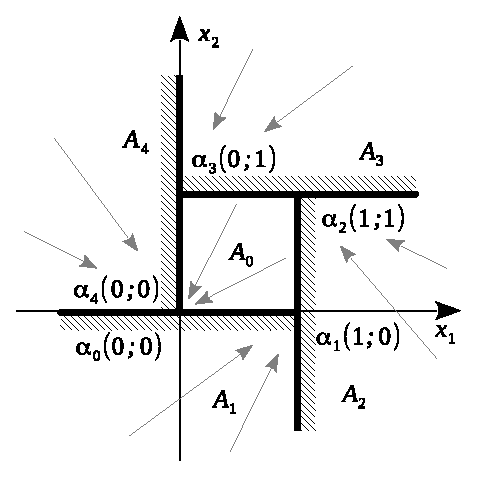
\includegraphics[width=0.4\linewidth]{quad3.eps}
	\caption{Разбиение плоскости, отмеченные точки и направления сдвигов}
	\label{fig:somelabel}
	%\vspace{2cm}
\end{figure}

Сразу заметим, что $\alpha_i \in \overline{A_i}$, $i=0,...,4$ и
$\alpha_i \in A_{i+1}$, $i=0,...,3$ (тогда как $\alpha_4 = \alpha_0 \in A_{1}$).

Таким образом, вся координатная плоскость оказалась разбита на четыре угла $A_1, ..., A_4$ и квадрат $A_0$.
Квадрат не включает свои границы; для каждого угла одна его сторона включается в угол,
а вторая сторона и вершина --- нет (они включаются в <<соседний>> угол).
Именно за счёт такого разбиения и достигается эффект примера.

В дальнейшим в случае, когда нижних индексов два, первый нижний индекс
будет отвечать за номер области и обозначаться через $i$,
$i=0, ..., 3$, второй --- за номер координаты
(или соответствующего ей уравнения) и обозначаться $j$, $j=1, 2$.

Рассмотрим систему двух обыкновенных дифференциальных уравнений
\begin{equation}\label{difur_primer_R2}
	\frac{dx_j(t)}{dt} = -\gamma_{ij}(x_j(t)-p_{ij})^2,
\end{equation}
где
$
	\gamma_{ij} = \operatorname{sgn}(x_j(0)-p_{ij}), j=1,2;
	(x_1, x_2) \in A_i,  \alpha_i = (p_{i1},p_{i2}).
$
Обратим внимание, что каждая координата меняется независимо от другой и гиперболически стремится
к некоторому предельному значению (это будет показано далее).

Для $\gamma_{ij} \neq 0$ решения этой системы на $[0, \infty)$ имеют вид
\begin{equation}\label{primer_R2_x_j}
	x_j(t) = \frac{\gamma_{ij}}{t+C_0}+p_{ij}, C_0 > 0,
\end{equation}
откуда
$
	x_j(t) \xrightarrow[t\to \infty ]{}{p_{ij}},
$
при этом знак разности $x_j(t) - p_{ij}$ не меняется.
Если же $\gamma_{ij}=0$, то по построению $x_j(0)=p_{ij}$,
и формула (\ref{primer_R2_x_j}) также верна.

Выпишем теперь оператор сдвига.
Положим в (\ref{primer_R2_x_j}) $t=0$, получим
$
	x_j(0) = \gamma_{ij}/{C_0}+p_{ij}
$.

Выразив отсюда $C_0$, подставим полученное выражение и выражение для $\gamma_{ij}$ в (\ref{primer_R2_x_j}).
Таким образом, оператор сдвига по траекториям уравнения (\ref{difur_primer_R2}) имеет вид
\begin{equation}\label{primer_R2_oper_sdviga}
	\tilde{S}_t(x_{j}(0)) = \frac{x_{j}(0)-p_{ij}}{|x_{j}(0)-p_{ij}|t+1}+p_{ij}
\end{equation}

Заметим, что числитель дроби не зависит от $t$, а знаменатель всегда строго положителен.
Следовательно, разность $\tilde{S}_t(x_j(0)) - p_{ij}$ сохраняет знак,
и траектория, начавшись в области $A_i$, никогда не перейдёт в другую область $A_{i'}$, $i \neq i'$.

Для $x_0 \in A_i$ имеем
\begin{equation}\label{primer_R2_stremlenie}
	S_t(x_0) \xrightarrow[t \to \infty]{} \alpha_{i},
\end{equation}
причём монотонно по $t$.
Действительно,
\begin{multline}
	\|S_t(x_0) - \alpha_i\| \leq
	\sqrt{2} \max_{j=1,2} \left| \frac{x_{j}(0)-p_{ij}}{|x_{j}(0)-p_{ij}|t+1} + p_{ij} - p_{ij}  \right| =
	\sqrt{2} \max_{j=1,2} \left| \frac{x_{j}(0)-p_{ij}}{|x_{j}(0)-p_{ij}|t+1} \right| \leq
	\\ \leq
	\sqrt{2} \max_{j=1,2} \left| \frac{x_{j}(0)-p_{ij}}{|x_{j}(0)-p_{ij}|t} \right| =
	\sqrt{2} \max_{j=1,2} \left| \frac{1}{t} \right| =
	\frac{\sqrt{2}}{t} \xrightarrow[t \to \infty]{} 0
\end{multline}

Заметим, что эта оценка равномерна по $x_{j}(0)$.
Более того, из того, что $\alpha_i \in A_{i+1}$, $i=0,...,3$,
следует, что $S_t(\alpha_i) \xrightarrow[t \to \infty]{} \alpha_{i+1}$,
т.~е. множество функций-констант
$$
	U = \{ u_i(t) \equiv \alpha_i \}_{i=0}^{3}
$$
не пересекается со множеством решений уравнения (\ref{difur_primer_R2}).

Покажем теперь, что $U$ --- траекторный аттрактор в смысле [\cite{Zelenaya}, опред. 3.2.3].
Компактность и ограниченность множества из четырёх функций-констант в пространствах
ы$C(\mathbb{R}_+; \mathbb{R}^2)$ и $L_\infty(\mathbb{R}_+; \mathbb{R}^2)$ очевидна.
Очевидно и то, что $U$ трансляционно инвариантно.

Осталось показать, что $U$ есть притягивающее множество в пространстве траекторий уравнения (\ref{difur_primer_R2}),
которое мы обозначим $H^+$.
Действительно, пусть $M>0$ и $B\subset H^+$ --- ограниченное в $L_\infty(\mathbb{R}_+; \mathbb{R}^2)$ множество.
Тогда
\begin{multline*}
	h_{C([0,M];\mathbb{R}^2)}(\Pi_M T(t)B,\Pi_M U) =
	\sup_{v\in B} \inf_{u\in U} \| T(t) v - u \|_{C([0,M];\mathbb{R}^2)} =
	\\ =
	\sup_{v\in B} \min_{i=0,..,3} \| T(t) v - u_i \|_{C([0,M];\mathbb{R}^2)} =
	\sup_{v\in B} \min_{i=0,..,3} \max_{s\in[0,M]} \| (T(t) v)(s) - u_i(s) \| =
	\\ =
	\sup_{v\in B} \min_{i=0,..,3} \max_{s\in[0,M]} \| (T(t) v)(s) - \alpha_i \| =
	\sup_{v\in B} \min_{i=0,..,3} \max_{s\in[t,t+M]} \| v(s) - \alpha_i \| \leq
	\frac{\sqrt{2}}{t} \xrightarrow[t\to + \infty]{} 0
\end{multline*}
Таким образом, $U$ --- действительно траекторный аттрактор, пересечение которого с пространством траекторий
уравнения (\ref{difur_primer_R2}) пусто.

\section{}

Покажем теперь, что глобального аттрактора полугруппы трансляций
в смысле динамической системы в данном примере не существует.
Предположим противное, т.е. что существует $P$ --- глобальный аттрактор полугруппы трансляций,
порождаемой оператором сдвига (\ref{primer_R2_oper_sdviga}).

Пусть сначала $\exists(i=0,...,4)[\alpha_i \notin P]$.
В силу определения глобального аттрактора полугруппы трансляций
$P$ компактно в $\mathbb{R}^2$.
Тогда расстояние $\rho$ от $P$ до $\alpha_i$ положительно.

Положим $\varepsilon = \frac{\rho}{3} > 0$ и покажем,
что условие притяжения из определения аттрактора полугруппы трансляций не выполняется.

Рассмотрим $V_\varepsilon = A_i \cap B(\alpha_i, \varepsilon)$ и некоторое решение $x_\varepsilon(t)$
такое, что $x_\varepsilon(0) \in V_\varepsilon$.
Тогда в силу монотонности стремления (\ref{primer_R2_stremlenie})
$\forall(t>0)[x_\varepsilon(t) \in V_\varepsilon]$.
Но $V_\varepsilon$ отделено от $P$, следовательно, $x_\varepsilon{t}$ не попадает в $\varepsilon$--окрестность $P$
ни при каких положительных $t$, что доказывает нарушение условия притяжения.

Значит, если аттрактор $P$ полугруппы трансляций существует, то $\alpha_i \in P, i=0,...,4$.
Но тогда $\forall(t>0)[S_t P \ne P]$.
Действительно, траектория, выходящая из $\alpha_i$, стремится к $\alpha_{i+1}$;
а все траектории, выходящие из точек области $A_i$, стремятся к $\alpha_i$,
но никогда не достигают её.

Следовательно, аттрактора полугруппы трансляций в данном случае не существует.
